% vim:encoding=utf8 ft=tex sts=2 sw=2 et:
% Copyright (c) 2009 Jaroslaw Koszuk
%
% $Id$

\documentclass{tewiart}

\usepackage[utf8]{inputenc}
\usepackage[T1]{fontenc}
\usepackage{graphicx}
\usepackage{amsthm}
\usepackage{amsmath}
\usepackage{txfonts}
\usepackage{epstopdf}
\usepackage{placeins}
\usepackage[english]{babel}
\usepackage[utf8]{inputenc}
\usepackage[table]{xcolor}
\usepackage{array}
\usepackage{subcaption}
\usepackage{hyperref}

\newtheorem{definition}{Definition}
\newtheorem{theorem}[definition]{Theorem}
\newtheorem{corollary}[definition]{Corollary}
\newtheorem{proposition}[definition]{Proposition}
\newtheorem{example}[definition]{Example}


\title{Study on the effectiveness of the investment strategy based on a classifier with rules adapted by machine learning}
\headtitle{}
\author{Wiliński A.\inst{1}, Bera A.\inst{1}, Nowicki W.\inst{1}, Błaszyński P.\inst{1}}
\headauthor{Wiliński A., Bera A. et al.}
\affiliation{%
  \inst{1}West Pomeranian University of Technology,Szczecin, Poland\\
  \{awilinski, abera, wnowicki, pblaszynski\}@wi.zut.edu.pl
}
\keywords{machine learning,  cross validation, pattern recognition, classification, investment strategy, algotrading, forecasting, time series}

\begin{document}

\maketitle

\begin{abstract}
In this paper authors examine two transactional strategies based on the classifier which opens positions using some rules and closes them using different rules. A rule set contains time-varying parameters that when matched allow to make an investment decision. Researches contain the study of variability of these parameters and the relationship between learning period and testing (using the learned parameters). The strategies are evaluated based on the time series of cumulative profit achieved in the test periods. The study was conducted on the most popular currency pair EURUSD sampled with interval of 1 hour.
\end{abstract}

\section{Introduction}
The aim of this work is to verify the hypothesis of the possibility of extracting patterns from time series, that would be classifiable as those that provide more accurate and better statistic prognosis. Another important objective is to confirm the assumption, that the time series of financial markets have a "memory" about the effectiveness of the learned pattern in a period after the learning one.  This approach is consistent with the classic aim of machine learning shown by K.Murphy’ego \cite{Murphy}, especially to financial markets described by Satchwell \cite{Satchwell}. Authors also intend to follow the principle of reproducibility of studies by other researchers, as well as by themselves, in other data environments, to make sense of the use of computational intelligence in its reasonable reproducibility \cite{Polya, Donoho}, in extracting of the regularity from chaos \cite{Ball, Pedrycz}. \\

The authors build an investment strategy with a relatively high complexity (measured by the number of factors included in the model), derived from a strategies group called strategy of simple rules (simple rules). In the literature those strategies are considered to be mainly strategies based on moving averages - their intersections and derivatives shown for example by Brock et al. \cite{Brock}, Cai et al. \cite{Cai} and many other authors \cite{Gencay, LeBaron, Tian}. Of course, the world of algorithms as well as prediction methods using a completely different nature, such as regression \cite{Muriel}, multiple regression \cite{Wilinski, Fujimoto}, Fourier and wavelet transforms, and many others \cite{Raghuraj, KleskWilinski} is plenteous. The authors use these methods as a basis for comparison, however they focus on mentioned simple rules.\\

Authors propose strategy, that differs by suggesting different behaviors than the ones proposed when using Bollinger's Band, which has its foundation in a band built in an unusual way. According to the strategy based on that band, generally it can be assumed that the trend is horizontal and it is recommended to open position to the center of the band, after its cross by the price from the inside. In proposed strategies, authors use another band that is based on maxima of the maxima and minima of the minima of last several candles.\\

In considered strategies authors move away from the principle of opening positions to the center of the band. In one modification, hereinafter referred to as sub strategy, position opens into the center of the band, whereas in another one, position opens on the outside. By treating the two considered sub strategies as an entirety and as strategies that are mutually retrieving (although a more appropriate word would be complementary) authors assume, that in the selected trading section, opening positions in opposite directions, of course not at the same time, can be done intentionally and effectively. During the trading, nature of the market (trend, volatility) may change. The market may be in some periods horizontal, in other trended. It is appropriate to seek all opportunities for profit. A similar philosophy is applied by several Krutsinger correspondents \cite{Krutsinger}, , who belong to most prominent traders in US, who advocate unfounded reversal of the direction of opening the positions in case of series of failures.\\

Returning to the issue of the complexity of the strategy, there are often opinions that the growing complexity of the prediction model is not indicated, because in learning section it  leads to overfitting \cite{Murphy, Cai, Fujimoto}  resulting in a greater error in the test sections. The problem of selecting the proper ratio between learning and testing phase is still unsolved for the non-stationary time series \cite{Ball, Ivakhnenko}. In this situation the right approach seems to be the use of the idea of computational intelligence \cite{Polya, Pedrycz} by which the empirical justification hypothesis entitles to use the model.\\

Therefore authors use two rather complex strategies (described below), achieving results that are in their assessment rewarding. They draw attention to the fact that the satisfaction problem belongs to the other sciences and depends on the trader's individual perception of the relationship between profit and risk, greed and fear \cite{Kahneman}. However, the issue of emotions in the trade is not considered here, but only noticed.\\

The tests were deliberately performed in a fragment of the time series of a heavily diversified course, which contains both rising and downward trends as well as horizontal elements (Fig. \ref{timeSeries}). It is the time series, consisting of 4734 1-hour candles, of the most important and the most fluent currency pair EURUSD from 22.10.2012.
\begin{figure}[h!]
\begin{center}
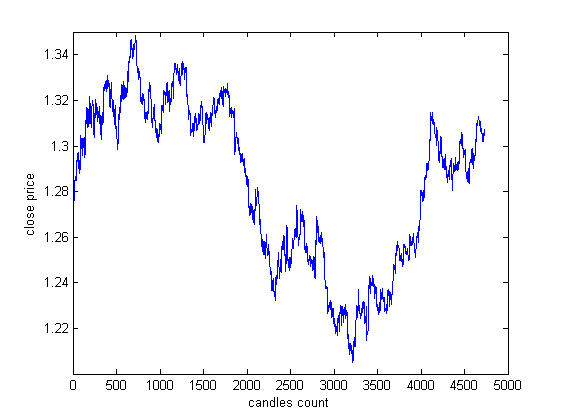
\includegraphics[width = 0.6\textwidth]{pictures/eurusd221012.png}
\end{center}
\caption{Time series EURUSD 1h}
\label{timeSeries}
\end{figure}
\FloatBarrier
%%%%%%%%%%%%%%%%%%%%%%%%%%%%%%%%%%%%%%%%%%%%%%%%%%%%%%%%
\section{Characteristics of investment strategies}
The objective of the two considered strategies is to make investment decisions about buying or selling - opening long or short position in the studied market - the currency pair EURUSD. Decision is based on intersection of the current price and one of two barriers of additional indicator, called the ribbon. The band is made of two values calculated at the opening of each candle on the basis of historical data of the market. During the candle values of the band do not change, therefore barriers are creating step functions. In case, when the current price exceeds any of the barrier values (goes out of the band), a decision to buy or sell is made - the type of decision depends on the variant of the considered strategy - decision for sub strategy TewiMiC is different than in case of TewiMiD. Names of the strategies are derived from the name of the project, in which the research was carried out.

\subsection{Definition of the band}
The value of barriers forming a band is calculated using the maximum and minimum values of the last candle (OHLC). In the case of the upper band, it is the maximum of the maximal values of the n last candles, whereas in the case of the bottom band, it is the minimum of the minimal values of m last candles. 

\begin{equation}
topBorder = \max{(H_{i-n},...,H_{i-1})}
\end{equation}
\begin{equation}
bottomBorder = \min{(L_{i-m},...,L_{i-1})}
\end{equation}

As mentioned earlier, strategy comes in two versions that differ in terms of opening the positions when crossing the band. These differences result from different investor assumption about currently prevailing market trend. In the first case it is believed that the trend has just started and positions need to be opened in accordance with it. In the second case, the play is against the trend. The two considered variants, TewiMiC and TewiMiD, are based on excesses of the lower limit of the band. TewiMiD implies existence of a downward trend, for which when crossing (down) the lower limit of the band, a short position (assuming the price drop) is opened. This is known it literature and in trading as Sell Stop model. \\

TewiMiC assumes the opposite case, therefore it is needed to open a long position (assuming the price increase).  This is Buy Limit model.

\subsection{Strategy parameters}
Considered strategies are based on a objects classification (events that meet the conditions contained in the set of rules which depend on the  value of certain parameters). Object - the event - is another candle. Rules are logical sentences like "if the price is greater than the upper barrier of the band", parameter is for example the upper barrier, which is a variable value. \\

These parameters will determine whether the strategy will earn or lose. Appropriate selection of parameter values is therefore a key optimization issue in the use of the strategy. Considered strategies have 11 parameters, which are subject of optimization.
\begin{itemize}
\item p1 --- the number of candles, based on which the calculation of the current value of the band barrier is made; for researched time series, value of p1 generally ranges from 10 to 30;
\item p2 --- number of steps forward, after which the position is closed in case none other close condition was met before; this value belongs to range from 3 to 40;
\item p3 --– StopLoss condition; usually it remained in range from 0.002 to 0.017 expressed in values of EURUSD, which in researched period stayed in range from 1.2 to 1.4, as can be seen in Fig. \ref{timeSeries};
\item p4 --– TakeProfit condition; generally ranged from 0.0015 to 0.009;
\item p5 --- band buffer, offset from the barrier of the band defining the actual level of the expected crossing of the  price; ranged from -0.002 to 0.003;
\item p6 --- maximum number of open positions at the same time; ranged from 3 to 20;
\item p7 --- number of candles that determines average volume value; generally ranged from 2 to 10;
\item p8 --- maximum value of the difference between the current value of the volume and the average value calculated on the basis of p7 candles back; ranged from 150 to 500;
\item p9 --- number of candles on the cumulative profit curve, based on which current drawdown is calculated; ranged from 5 to 25;
\item p10 --- highest acceptable drawdown on the cumulative yield curve; generally ranged from 0.0021 to 0.008;
\item p11 --- acceptable amount of the cumulative loss for all currently open positions; ranged from 0.0005 to 0.003;
\end{itemize}

\subsection{Conditions of opening}
As mentioned before, the signal to open the position is the intersection of the current price of the observed value and some barrier (that results from the calculated band). Special parameter called the buffer (p5) has been added, causing the offset of barrier from its actual value. Thus, the condition for opening TewiMIC strategy is: 
\begin{equation}
\begin{split}
if[(price < bottomBorder(p1) - buffor(p5)) \\ 
\text{and } (current p6 < p6) \text{ and } (Vol - meanVol(p7) < p8)] \\
\text{then open position long}
\end{split}
\end{equation}
where:\\
\textit{price} – current value for EURUSD;\\
\textit{bottomBorder(p1)} – value of lower band barrier for parameter p1; here minimum of last p1 minima; \\
\textit{buffor(p5)} – value of buffer that moves said barrier;\\
\textit{current p6} – number of currently opened positions;\\
\textit{Vol} – current value of volume (in the candle);\\
\textit{meanVol(p7)} – mean of volume of last p7 candles;\\

\noindent and the opening condition for TewiMiD is:
\begin{equation}
\begin{split}
if[(price < bottomBorder(p1) - buffor(p5)) \\ 
\text{and } (current p6 < p6) \text{ and } (Vol - meanVol(p7) > p8)] \\
\text{then open position short}
\end{split}
\end{equation}

As a result of these conditions, long positions, in sub strategy TewiMIC, are opened when three conditions are met simultaneously: crossing the bottom barrier reduced by buffer by the current price, the number of open positions is lesser than the limit (which is the optimized parameter p6) and the difference between the current volume and the average of the volume of the last p7 candle is less than the parameter p8.\\

For TewiMiD strategy, similar, with significant differences - short positions will be opened and it is advisable that current volume should be greater  than the average. As the result of conducted research, authors concluded that volume (number of price changes in observed time frame – here during one hour) was the most important and most sensitive factor of decision model.\\

These conditions can be met in two cases during the period of the current considered candle. They can be met immediately at the opening of the candle i.e. the opening value of the current candle is smaller than the barrier bottomBorder reduced by parameter p5. That condition can be met within the candle, when the current value of the price break through the lower barrier. \\

The result of that is that we have two distinctly different opening conditions.

\subsection{Conditions of closing}
In both sub strategies there are 7 cases of closing the open positions, which results in their complexity - both in terms of logic and calculation. This complexity, however, exhausts all the possible surprises and does not  leave any opportunity for the unexpected market behavior. Of course, depending on the values of the parameters, frequency occurrences of closure cases can be very different.\\

Firstly the terms for closing the long positions that were opened by conditions for TewiMiC will be presented.
\begin{enumerate}
\item Opened long position will be closed, if at the close of the candle \textit{(i + p2)} the position remained open, where \textit{i} - number of candle, which was opened;

\item Position will be closed if at the opening of the next (i + k)-th - the candle after i-th candle, in which the position was opened, following condition is met: 
\begin{equation}
PriceO(i+k)-Price(i) <-SL
\end{equation} 
where \textit{ProceO(i+k)} is the opening value for (i+k)-th candle;\\
Then the profit (in this case loss) will be calculated as:
\begin{equation}
Profit =PriceO (i+k)-Price(i);
\end{equation}

\item Position will be closed if inside the opening of the next (i + k)-th - the candle after i-th candle, in which the position was opened, following condition is met: 
\begin{equation}
(PriceO(i+k)-Price(i) )>-SL \text{ and } (LowPrice(i+k)-Price(i))<-SL
\end{equation} 
Then the profit (in this case loss) will be calculated as:
\begin{equation}
Profit =-SL;
\end{equation}

\item Position will be closed if at the opening of the next (i + k)-th - the candle after i-th candle, in which the position was opened, following condition is met: 
\begin{equation}
PriceO(i+k)-Price(i)>TP
\end{equation} 
Then the profit will be calculated as:
\begin{equation}
Profit =PriceO (i+k)-Price(i);
\end{equation}

\item Position will be closed if inside the opening of the next (i + k)-th - the candle after i-th candle, in which the position was opened, following condition is met: 
\begin{equation}
(PriceO(i+k)-Price(i) )<TP \text{ and } (HighPrice(i+k)-Price(i))>TP
\end{equation} 
Then the profit will be calculated as:
\begin{equation}
Profit =TP;
\end{equation}
where \textit{HighPrice(i+k)} is the maximum value for (i+k) candle;

\item Position will be closed if at the opening of the next (i + k)-th - the candle after i-th candle, in which the position was opened, following condition is met: 
\begin{equation}
PriceO(i+k) >topBorder(i+k)
\end{equation} 
Then the profit will be calculated as:
\begin{equation}
Profit =PriceO (i+k) -  Price(i) ;
\end{equation}

\item Position will be closed if inside the opening of the next (i + k)-th - the candle after i-th candle, in which the position was opened, following condition is met: 
\begin{equation}
Price(i+k) >topBorder(i+k)
\end{equation} 
Then the profit will be calculated as:
\begin{equation}
Profit =topBorder (i+k) -  Price(i) ;
\end{equation}

\end{enumerate}

In sub strategy TewiMiD conditions will look slightly different.
\begin{enumerate}
\item Opened short position will be closed if at the close of the candle (i + p2)-th the position remained open;\\
Position will be closed if at the opening of the next (i + k)-th - the candle after i-th candle, in which the position was opened, following condition is met:
\begin{equation}
Price(i)-PriceO(i+k)<-SL
\end{equation}                                      
Then the profit (in this case loss) will be calculated as:
\begin{equation}
Profit =-PriceO (i+k) +  Price(i) ;
\end{equation}

\item Position will be closed if inside the opening of the next (i + k)-th - the candle after i-th candle, in which the position was opened, following condition is met:
\begin{equation}
(-PriceO (i+k)+price(i) )>-SL \text{ and } (-HighPrice(i+k)+Price(i))<-SL
\end{equation}                          
Then the profit (in this case loss) will be calculated as:
\begin{equation}
Profit =-SL; 
\end{equation}

\item Position will be closed if at the opening of the next (i + k)-th - the candle after i-th candle, in which the position was opened, following condition is met:
\begin{equation}
Price(i)-PriceO(i+k>TP
\end{equation}                                           
Then the profit will be calculated as:
\begin{equation}
Profit =-PriceO (i+k)  + Price(i) ;
\end{equation} 


\item Position will be closed if inside the opening of the next (i + k)-th - the candle after i-th candle, in which the position was opened, following condition is met: 
\begin{equation}
(-PriceO(i+k)+price(i) )<TP \text{ and } (-LowPrice(i+k)+Price(i))>TP
\end{equation}
Then the profit will be calculated as:
\begin{equation}
Profit =TP; 
\end{equation}

\item Position will be closed if at the opening of the next (i + k)-th - the candle after i-th candle, in which the position was opened, following condition is met: 
\begin{equation}
PriceO(i+k) >bottomBorder(i+k)
\end{equation}                          
Then the profit will be calculated as:
\begin{equation}
Profit =-PriceO (i+k)  + Price(i) ;
\end{equation}

\item Position will be closed when inside the opening of the next (i + k)-th - the candle after i-th candle, in which the position was opened, following condition is met:
\begin{equation}
Price(i+k) >bottomBorder(i+k)
\end{equation}                           
Then the profit (in this case loss) will be calculated as:
\begin{equation}
Profit =-bottomBorder (i+k) +  Price(i) ;
\end{equation}

\end{enumerate}
Additional conditions that are checked with each closing are the rules containing parameters p9, p10, p11. These parameters are found in the rules limiting the risk of an unacceptable failure. Moreover, the principle stating that in the case when the opening took place at the beginning of the candle, it is permissible to keep it open until following candle is opened was used. Because of that,  it was possible to avoid ambiguity involving the unpredictable sequence of the SL and TP.


%%%%%%%%%%%%%%%%%%%%%%%%%%%%%%%%%%%%%%%%%%
\section{Badanie strategii}
\begin{figure}[h!]
\begin{center}
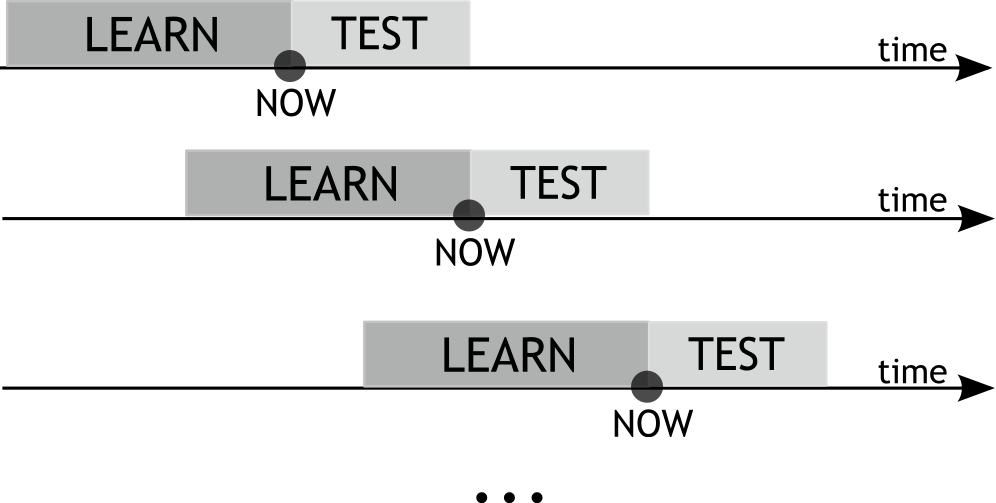
\includegraphics[width=0.6\textwidth]{pictures/metodyka_badan.png}
\caption{Metodyka przeprowadzonych badań dla przypadku zmiennego okna testowego}
\label{metodyka}
\end{center}
\end{figure}
\FloatBarrier

\begin{figure}[h!]
\begin{center}
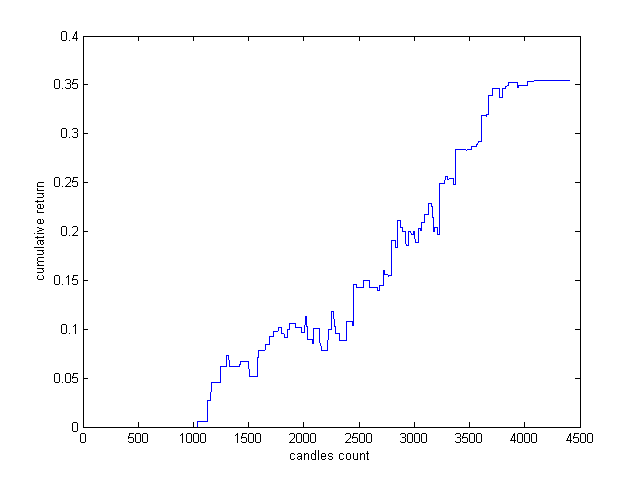
\includegraphics[width=0.7\textwidth]{pictures/mic_100.png}
\caption{PODPIS}
\label{MiC100}
\end{center}
\end{figure}
\FloatBarrier

\begin{figure}[h!]
\begin{center}
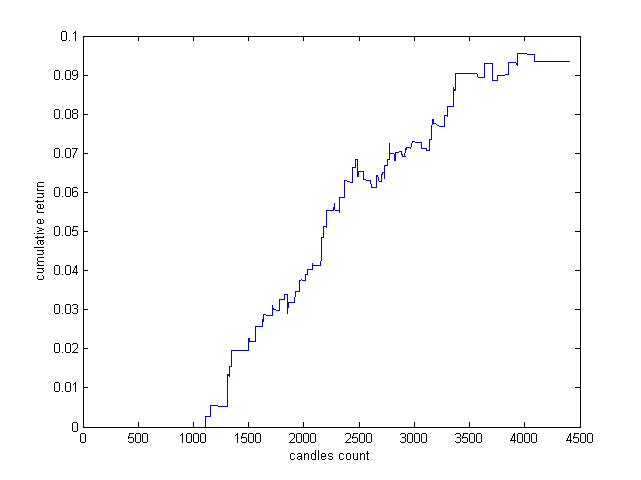
\includegraphics[width=0.7\textwidth]{pictures/mid_100.png}
\caption{PODPIS}
\label{MiD100}
\end{center}
\end{figure}
\FloatBarrier

\begin{figure}[h!]
\begin{center}
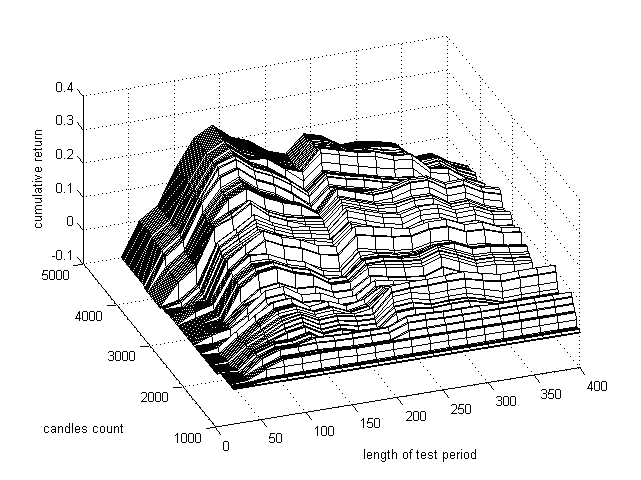
\includegraphics[width=0.7\textwidth]{pictures/cumulativeReturnsC.png}
\caption{PODPIS}
\label{Cum3DMiC}
\end{center}
\end{figure}
\FloatBarrier

\begin{figure}[h!]
\begin{center}
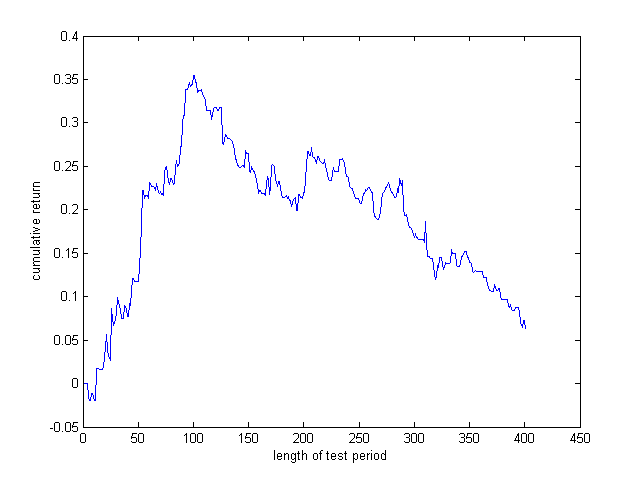
\includegraphics[width=0.7\textwidth]{pictures/mic_end.png}
\caption{PODPIS}
\label{Cum3DMiCend}
\end{center}
\end{figure}
\FloatBarrier

\begin{figure}[h!]
\begin{center}
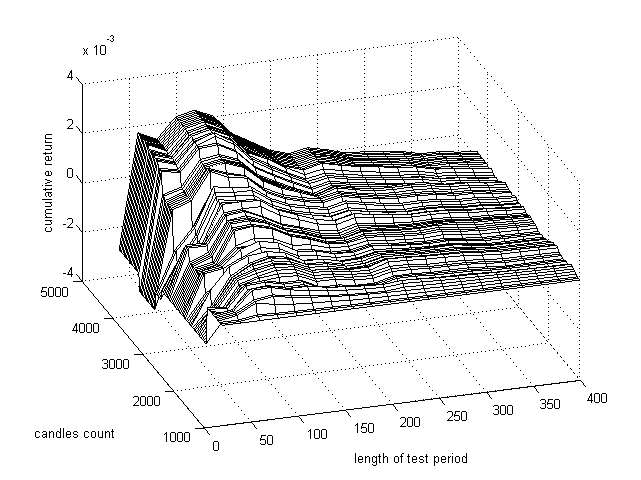
\includegraphics[width=0.7\textwidth]{pictures/cumulativeReturnsPerCandleC.png}
\caption{PODPIS}
\label{Cum3DPerCMiC}
\end{center}
\end{figure}
\FloatBarrier

\begin{figure}[h!]
\begin{center}
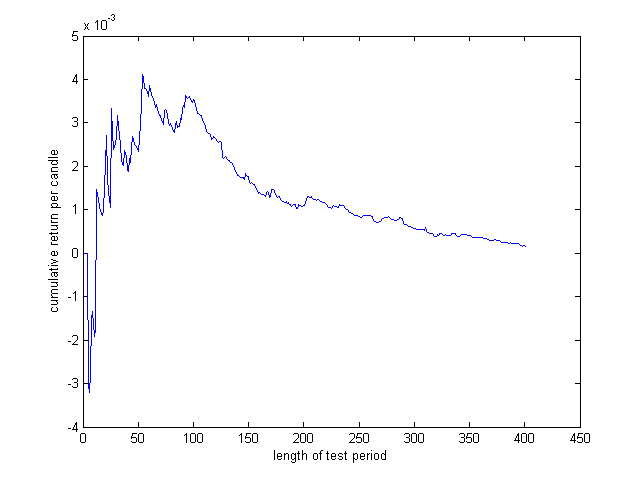
\includegraphics[width=0.7\textwidth]{pictures/mic_percandle_end.png}
\caption{PODPIS}
\label{Cum3DPerCMiCend}
\end{center}
\end{figure}
\FloatBarrier

\begin{table}[h!] 
\caption{TABLE 1}
\label{table1}
 \begin{tabular}{|l|l|l|l|l|l|} 
 \hline size & profit & profit per canlde & Calmar & Open positions & Percentage [\%]\\ \hline  
10 & -0.0192 & -0.0019 & -0.728 & 34 & 10.97 \\ 
 20 & 0.0415 & 0.0021 & 2.1594 & 66 & 10.65 \\ 
 30 & 0.0812 & 0.0027 & 2.4182 & 93 & 10 \\ 
 40 & 0.0768 & 0.0019 & 1.4048 & 120 & 9.68 \\ 
 50 & 0.1176 & 0.0024 & 2.4069 & 134 & 8.65 \\ 
 60 & 0.2318 & 0.0039 & 5.3914 & 153 & 8.23 \\ 
 70 & 0.2211 & 0.0032 & 4.7859 & 176 & 8.11 \\ 
 80 & 0.2359 & 0.0029 & 5.1063 & 196 & 7.9 \\ 
 90 & 0.3005 & 0.0033 & 8.6589 & 221 & 7.92 \\ 
 100 & 0.3548 & 0.0035 & 10.221 & 245 & 7.9 \\ 
 110 & 0.3294 & 0.003 & 9.4905 & 262 & 7.68 \\ 
 120 & 0.3172 & 0.0026 & 8.6479 & 283 & 7.61 \\ 
 130 & 0.2854 & 0.0022 & 4.5295 & 304 & 7.54 \\ 
 140 & 0.2512 & 0.0018 & 4.3911 & 335 & 7.72 \\ 
 150 & 0.2648 & 0.0018 & 4.6295 & 345 & 7.42 \\ 
 200 & 0.2194 & 0.0011 & 2.8244 & 482 & 7.77 \\ 
 250 & 0.2091 & 0.0008 & 2.2352 & 574 & 7.41 \\ 
 300 & 0.1684 & 0.0006 & 1.5345 & 720 & 7.74 \\ 
 350 & 0.1399 & 0.0004 & 1.0402 & 804 & 7.41 \\ 
 400 & 0.073 & 0.0002 & 0.5074 & 914 & 7.37 \\ 
 \hline \end{tabular} 
 \end{table}
 \FloatBarrier

%%%%%%%%%
\begin{figure}[h!]
\begin{center}
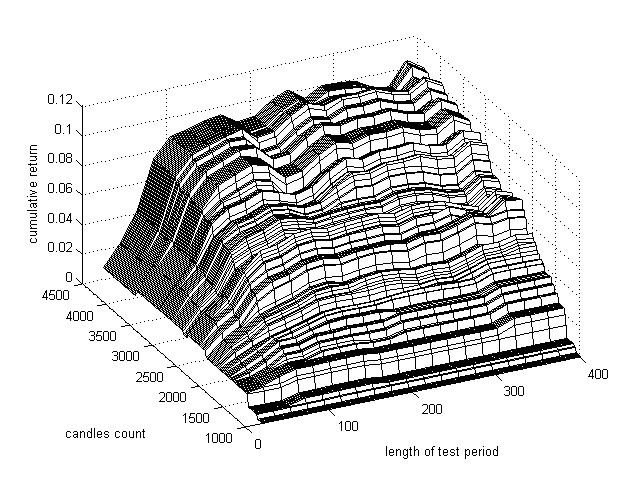
\includegraphics[width=0.7\textwidth]{pictures/cumulativeReturnsD.png}
\caption{PODPIS}
\label{Cum3DMiD}
\end{center}
\end{figure}
\FloatBarrier

\begin{figure}[h!]
\begin{center}
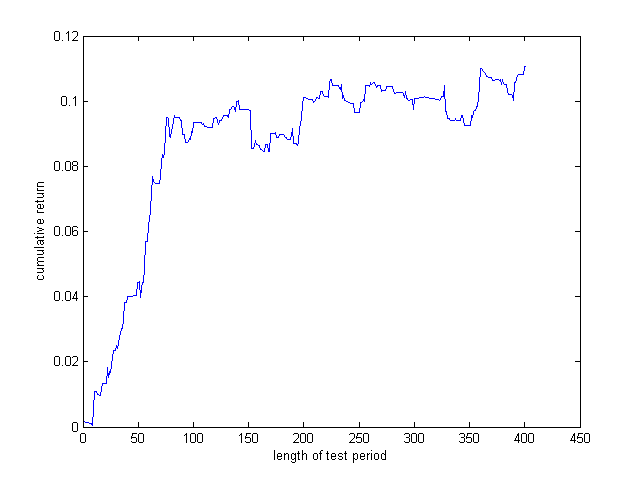
\includegraphics[width=0.7\textwidth]{pictures/mid_end.png}
\caption{PODPIS}
\label{Cum3DMiDend}
\end{center}
\end{figure}
\FloatBarrier

\begin{figure}[h!]
\begin{center}
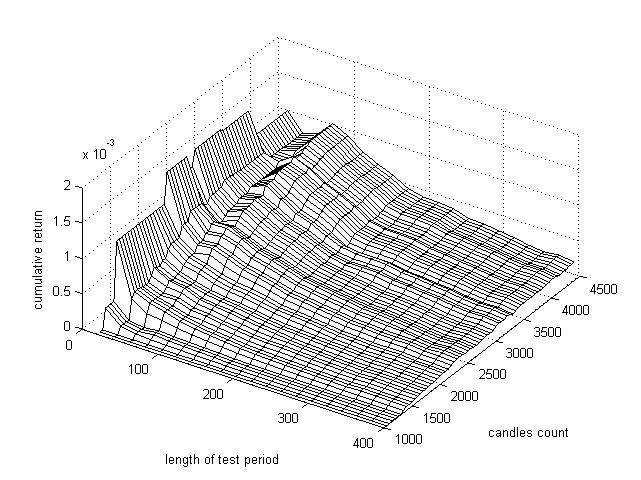
\includegraphics[width=0.7\textwidth]{pictures/cumulativeReturnsPerCandleD.png}
\caption{PODPIS}
\label{Cum3DPerCMiD}
\end{center}
\end{figure}
\FloatBarrier

\begin{figure}[h!]
\begin{center}
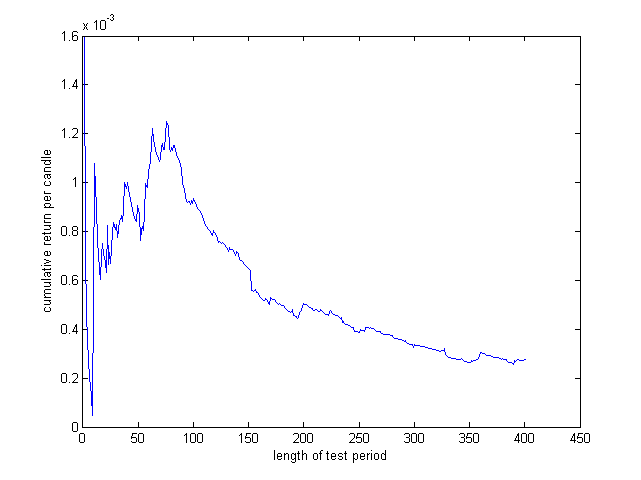
\includegraphics[width=0.7\textwidth]{pictures/mid_percandle_end.png}
\caption{PODPIS}
\label{Cum3DPerCMiDend}
\end{center}
\end{figure}
\FloatBarrier

\begin{table}[h!]
\caption{TABLE 2}
\label{table2}
 \begin{tabular}{|l|l|l|l|l|l|} 
 \hline size & profit & profit per canlde & Calmar & Open positions & Percentage [\%]\\ \hline  
10 & 0.0108 & 0.0011 & 2.3305 & 11 & 3.55 \\ 
 20 & 0.0135 & 0.0007 & 2.4981 & 20 & 3.23 \\ 
 30 & 0.0249 & 0.0008 & 4.2953 & 47 & 5.05 \\ 
 40 & 0.0401 & 0.001 & 8.012 & 60 & 4.84 \\ 
 50 & 0.0443 & 0.0009 & 8.868 & 66 & 4.26 \\ 
 60 & 0.0636 & 0.0011 & 13.25 & 83 & 4.46 \\ 
 70 & 0.0771 & 0.0011 & 16.0687 & 95 & 4.38 \\ 
 80 & 0.0914 & 0.0011 & 19.0396 & 118 & 4.76 \\ 
 90 & 0.0899 & 0.001 & 10.5222 & 130 & 4.66 \\ 
 100 & 0.0935 & 0.0009 & 12.7934 & 141 & 4.55 \\ 
 110 & 0.0921 & 0.0008 & 12.6559 & 150 & 4.4 \\ 
 120 & 0.0949 & 0.0008 & 13.0337 & 159 & 4.27 \\ 
 130 & 0.0955 & 0.0007 & 13.1243 & 178 & 4.42 \\ 
 140 & 0.0998 & 0.0007 & 11.5503 & 188 & 4.33 \\ 
 150 & 0.0974 & 0.0006 & 9.6789 & 194 & 4.17 \\ 
 200 & 0.1011 & 0.0005 & 9.464 & 263 & 4.24 \\ 
 250 & 0.0965 & 0.0004 & 9.0392 & 328 & 4.23 \\ 
 300 & 0.1008 & 0.0003 & 9.3983 & 410 & 4.41 \\ 
 350 & 0.0924 & 0.0003 & 7.2935 & 467 & 4.3 \\ 
 400 & 0.1105 & 0.0003 & 8.1655 & 558 & 4.5 \\ 
 \hline \end{tabular} 
 \end{table}
 \FloatBarrier
\bibliography{references-tewi}
\bibliographystyle{aiaa-tewi}


\end{document}